%!Tex Root=**/main.tex

\documentclass[
    10pt,
    aspectratio=1610,
    xcolor={dvipsnames,pst},
    % handout
]{beamer}
\usetheme[
    % subsectionpage=progressbar,
    progressbar=frametitle,
    block=fill
]{moloch}
% \mode<presentation>

\usepackage{pgfpages}
% \pgfpagesuselayout{2 on 1}[a4paper,border shrink=5mm]
% \pgfpagesuselayout{4 on 1}[a4paper,landscape,border shrink=5mm]
%%%%%%%%%%%%%%%%%%%%%%%%%%%%%%%%%%%%%%%%%%%%%%%%%%%%%%%%%%%%%%%%%%%%%%%%%%%%%%%%
%%%%%%%%%%%%% personal modification of the moloch/metropolis theme %%%%%%%%%%%%%
%%%%%%%%%%%%%%%%%%%%%%%%%%%%%%%%%%%%%%%%%%%%%%%%%%%%%%%%%%%%%%%%%%%%%%%%%%%%%%%%
% frametitle with right-aligned "section, subsection"
\newenvironment{Frame}[1]{
    \begin{frame}{#1 \hspace{0pt plus 1filll} \scriptsize \(\triangleleft\)\;\subsecname\;\(\triangleleft\)\;\secname}\vspace*{\fill}
}{\vspace*{\fill}\end{frame}}

% inner theme
\useinnertheme{rectangles}

% color palette
\definecolor{um-blue}{HTML}{002855}
\definecolor{um-gold}{HTML}{84754E}
\definecolor{um-red}{HTML}{Ef3340}
\definecolor{um-yellow}{HTML}{84754E}
% color theme
\colorlet{color-frametitle}{um-blue}
\colorlet{color-progressbar}{um-gold}

\setbeamercolor{frametitle}{fg=black!2, bg=color-frametitle}
\setbeamercolor{progress bar}{fg=color-progressbar, bg=color-progressbar!20}
\setbeamercolor{item projected}{fg=black!2, bg=color-progressbar}
\setbeamercolor{itemize item}{fg=color-progressbar}

% make progress bar's width larger
\makeatletter
\setlength{\moloch@titleseparator@linewidth}{2.5pt}
\setlength{\moloch@progressonsectionpage@linewidth}{2.5pt}
\setlength{\moloch@progressinheadfoot@linewidth}{2.5pt}
\makeatother

% make footnotesize smaller
\let\oldfootnotesize\footnotesize
\renewcommand*{\footnotesize}{\oldfootnotesize\tiny}

% footnote without counter
\newcommand\blfootnote[1]{%
  \begingroup
  \renewcommand\thefootnote{}\footnote{#1}%
  \addtocounter{footnote}{-1}%
  \endgroup
}

% footnotetext without counter
\newcommand\blfootnotetext[1]{%
  \begingroup
  \renewcommand\thefootnotetext{}\footnotetext{#1}%
  \addtocounter{footnotetext}{-1}%
  \endgroup
}

%%%%%%%%%%%%%%%%%%%%%%%%%%%%%%%%%%%%%%%%%%%%%%%%%%%%%%%%%%%%%%%%%%%%%%%%%%%%%%%%
%%%%%%%%%%%%%%%%%%%%%%%%%%%%%%%%%%%% fonts %%%%%%%%%%%%%%%%%%%%%%%%%%%%%%%%%%%%%
%%%%%%%%%%%%%%%%%%%%%%%%%%%%%%%%%%%%%%%%%%%%%%%%%%%%%%%%%%%%%%%%%%%%%%%%%%%%%%%%
\usepackage{xeCJK}
\setCJKmainfont{思源宋体}
\setCJKsansfont{思源黑体}
\setCJKmonofont{思源等宽}

%%%%%%%%%%%%%%%%%%%%%%%%%%%%%%%%%%%%%%%%%%%%%%%%%%%%%%%%%%%%%%%%%%%%%%%%%%%%%%%%
%%%%%%%%%%%%%%%%%%%%%%%%%%%%%%%%%%%% color %%%%%%%%%%%%%%%%%%%%%%%%%%%%%%%%%%%%%
%%%%%%%%%%%%%%%%%%%%%%%%%%%%%%%%%%%%%%%%%%%%%%%%%%%%%%%%%%%%%%%%%%%%%%%%%%%%%%%%
\definecolorseries{marknode-color-series}{hsb}{last}[hsb]{0.0,0.12,0.95}[hsb]{0.95,0.12,0.95}
\definecolorseries{annotation-color-series}{hsb}{last}[hsb]{0.0,0.85,0.6}[hsb]{0.95,0.85,0.6}
\resetcolorseries[8]{marknode-color-series}
\resetcolorseries[8]{annotation-color-series}

%%%%%%%%%%%%%%%%%%%%%%%%%%%%%%%%%%%%%%%%%%%%%%%%%%%%%%%%%%%%%%%%%%%%%%%%%%%%%%%%
%%%%%%%%%%%%%%%%%%%%%%%%%%%%%%%%%%%% glyph %%%%%%%%%%%%%%%%%%%%%%%%%%%%%%%%%%%%%
%%%%%%%%%%%%%%%%%%%%%%%%%%%%%%%%%%%%%%%%%%%%%%%%%%%%%%%%%%%%%%%%%%%%%%%%%%%%%%%%
\usepackage{fontawesome5}
\usepackage{bbding}
\usepackage{pifont}
\newcommand{\cmark}{\ding{51}}
\newcommand{\xmark}{\ding{55}}
\usepackage{romannum}
\usepackage{stmaryrd} % for \mapsfrom (inverse of \mapsto)

%%%%%%%%%%%%%%%%%%%%%%%%%%%%%%%%%%%%%%%%%%%%%%%%%%%%%%%%%%%%%%%%%%%%%%%%%%%%%%%%
%%%%%%%%%%%%%%%%%%%%%%%%%%%%%%%%%%%% table %%%%%%%%%%%%%%%%%%%%%%%%%%%%%%%%%%%%%
%%%%%%%%%%%%%%%%%%%%%%%%%%%%%%%%%%%%%%%%%%%%%%%%%%%%%%%%%%%%%%%%%%%%%%%%%%%%%%%%
\usepackage{booktabs}

% ref: https://tex.stackexchange.com/a/614273/240783
\usepackage{tabularray}
\UseTblrLibrary{booktabs}

%%%%%%%%%%%%%%%%%%%%%%%%%%%%%%%%%%%%%%%%%%%%%%%%%%%%%%%%%%%%%%%%%%%%%%%%%%%%%%%%
%%%%%%%%%%%%%%%%%%%%%%%%%%%%%%%%%%% caption %%%%%%%%%%%%%%%%%%%%%%%%%%%%%%%%%%%%
%%%%%%%%%%%%%%%%%%%%%%%%%%%%%%%%%%%%%%%%%%%%%%%%%%%%%%%%%%%%%%%%%%%%%%%%%%%%%%%%
\usepackage{caption}
\captionsetup{font={scriptsize},
              labelfont={scriptsize},
              textfont={scriptsize},
              % hypcap=false,
              % format=hang,
              % margin=1cm
             }

%%%%%%%%%%%%%%%%%%%%%%%%%%%%%%%%%%%%%%%%%%%%%%%%%%%%%%%%%%%%%%%%%%%%%%%%%%%%%%%%
%%%%%%%%%%%%%%%%%%%%%%%%%%%%%%%%%%% graphics %%%%%%%%%%%%%%%%%%%%%%%%%%%%%%%%%%%
%%%%%%%%%%%%%%%%%%%%%%%%%%%%%%%%%%%%%%%%%%%%%%%%%%%%%%%%%%%%%%%%%%%%%%%%%%%%%%%%
% \usepackage{graphicx} % pre-loaded by beamer
\graphicspath{{../images}}

\usepackage{forest} % mindmap

% \usetikzlibrary{calc,tikzmark,arrows.meta,fit,positioning,decorations.markings}

%%%%%%%%%%%%%%%%%%%%%%%%%%%%%%%%%%%%%%%%%%%%%%%%%%%%%%%%%%%%%%%%%%%%%%%%%%%%%%%%
%%%%%%%%%%%%%%%%%%%%%%%%% equation annotation by TikZ %%%%%%%%%%%%%%%%%%%%%%%%%%
%%%%%%%%%%%%%%%%%%%%%%%%%%%%%%%%%%%%%%%%%%%%%%%%%%%%%%%%%%%%%%%%%%%%%%%%%%%%%%%%
% \usepackage{tikz}
% \usepackage[dvipsnames]{xcolor}
\usetikzlibrary{calc,tikzmark}
% \usepackage{tcolorbox}
\usepackage{makecell}
\usepackage{xstring}
%%%%%%%%%%%%%%%%%%%%%%%%%%%%%%%%%%%%%%%%%%%%%%%%%%%%%%%%%%%%%%%%%%%%%%%%%%%%%%%%
% Usage:
% \annotatedEquation{1: color/colorseries}{2: node name}{3: node direction}{4: x shift}{5: y shift}{6: anchor direction}{7: color/colorseries name}{8: annotation}{9: baseline direction}
%%%%%%%%%%%%%%%%%%%%%%%%%%%%%%%%%%%%%%%%%%%%%%%%%%%%%%%%%%%%%%%%%%%%%%%%%%%%%%%%
\newenvironment{annotatedEquationEnv}{
    \begin{tikzpicture}[
        overlay, remember picture,
        >=stealth, <-,
        nodes={align=left,inner ysep=1pt},
    ]
}
{
    \end{tikzpicture}
}
\newcommand*{\annotatedEquation}[9]{%
     \IfEqCase{#1}{%
        {color}{%
            \path (#2.#3) ++ (#4,#5) node [anchor=#6] (#2-annotate) { \color{#7} \scriptsize \makecell[l]{#8} };%
            \draw [#7] (#2.#3) |- (#2-annotate.south #9);%
        }%
        {colorseries}{%
            \path (#2.#3) ++ (#4,#5) node [anchor=#6] (#2-annotate) { \color{#7!!} \scriptsize \makecell[l]{#8} };%
            \draw [#7!!] (#2.#3) |- (#2-annotate.south #9);%
            \textcolor{#7!!+}{}%
        }%
    }[\PackageError{annotatedEquation}{Undefined option to annotatedEquation #1}{}]%
}%

%%%%%%%%%%%%%%%%%%%%%%%%%%%%%%%%%%%%%%%%%%%%%%%%%%%%%%%%%%%%%%%%%%%%%%%%%%%%%%%%
%%%%%%%%%%%%%%%%%%%%%%%%%% figure annotation by TikZ  %%%%%%%%%%%%%%%%%%%%%%%%%%
%%%%%%%%%%%%%%%%%%%%%%%%%%%%%%%%%%%%%%%%%%%%%%%%%%%%%%%%%%%%%%%%%%%%%%%%%%%%%%%%
% \usepackage{tikz}
%%%%%%%%%%%%%%%%%%%%%%%%%%%%%%%%%%%%%%%%%%%%%%%%%%%%%%%%%%%%%%%%%%%%%%%%%%%%%%%%
% Usage:
% \begin{annotatedFigureEnv}
%     {\includegraphics[width=0.5\linewidth]{example-image}}
%     \annotatedFigureBox{bottom-left}{top-right}{label}{label-position}
% \end{annotatedFigureEnv}
% Usage:
% \annotatedFigure{bottom-left}{top-right}{label}{label-position}
% Usage:
% \annotatedFigureImpl{1: bottom-left}{2: top-right}{3: label}{4: label-position}{5: box-color}{6: label-color}{7: border-color}{8: text-color}
% Usage:
% \figureBox{bottom-left}{top-right}{color}{thickness}
%%%%%%%%%%%%%%%%%%%%%%%%%%%%%%%%%%%%%%%%%%%%%%%%%%%%%%%%%%%%%%%%%%%%%%%%%%%%%%%%
\newcommand*\annotatedFigureImpl[8]{
    \draw [#5, ultra thick] (#1) rectangle (#2);
    \node at (#4) [fill=#6, thick, shape=rectangle, draw=#7, inner sep=2.5pt, font=\small\sffamily, text=#8] { #3 };
}
\newcommand*\annotatedFigure[4]{
    \annotatedFigureImpl{#1}{#2}{#3}{#4}{color-progressbar}{color-progressbar}{color-progressbar}{black!2}
}
\newcommand*\annotatedFigureText[4]{
    \node[draw=none, anchor=south west, text=#2, inner sep=0, text width=#3\linewidth,font=\sffamily] at (#1) {#4};
}
\newenvironment{annotatedFigureEnv}[1]{
    \centering
    \begin{tikzpicture}
        \node[anchor=south west,inner sep=0] (image) at (0,0) { #1 };
        \begin{scope}[x={(image.south east)},y={(image.north west)}]
}
{
        \end{scope}
    \end{tikzpicture}
}
\newcommand*\figureBox[4]{\draw[#3,#4,rounded corners] (#1) rectangle (#2);}


%%%%%%%%%%%%%%%%%%%%%%%%%%%%%%%%%%%%%%%%%%%%%%%%%%%%%%%%%%%%%%%%%%%%%%%%%%%%%%%%
%%%%%%%%%%%%%%%%%%%%%%%%%%%%%%% Taxonomy by TikZ %%%%%%%%%%%%%%%%%%%%%%%%%%%%%%%
%%%%%%%%%%%%%%%%%%%%%%%%%%%%%%%%%%%%%%%%%%%%%%%%%%%%%%%%%%%%%%%%%%%%%%%%%%%%%%%%
% ref: https://tex.stackexchange.com/a/112471/240783
% ref: https://tex.stackexchange.com/a/357412/240783
%%%%%%%%%%%%%%%%%%%%%%%%%%%%%%%%%%%%%%%%%%%%%%%%%%%%%%%%%%%%%%%%%%%%%%%%%%%%%%%%
\usetikzlibrary{shadows}
\makeatletter
\def\tikzopacityregister{.2} % the opacity of the shadows
\tikzset{
  opacity/.append code={
    \pgfmathsetmacro\tikzopacityregister{#1*\tikzopacityregister}
  },
  opacity aux/.code={ % this is the original definition of opacity
    \tikz@addoption{\pgfsetstrokeopacity{#1}\pgfsetfillopacity{#1}}
  },
  every shadow/.style={opacity aux=\tikzopacityregister}
}
\makeatother
\tikzset{
    my node for tree/.style={
            text=black,
            draw=lightgray!50,
            fill=lightgray!20,
            % inner color=lightgray!5,
            % outer color=lightgray!20,
            thick,
            minimum width=12mm,
            minimum height=6mm,
            rounded corners=3,
            text height=1.5ex,
            text depth=0ex,
            font={\sffamily},
            drop shadow,
        },
    invisible/.style={opacity=0,text opacity=0},
    visible on/.style={alt=#1{}{invisible}},
    alt/.code args={<#1>#2#3}{%
      \alt<#1>{\pgfkeysalso{#2}}{\pgfkeysalso{#3}} % \pgfkeysalso doesn't change the path
    },
}
\forestset{
    visible on/.style={
        for tree={
            /tikz/visible on={#1},
            edge+={/tikz/visible on={#1}},
        }
    },
    my tree/.style={
            my node for tree,
            s sep+=4pt,
            l sep+=10pt,
            grow'=east,
            edge+={lightgray},
            parent anchor=east,
            child anchor=west,
            edge path={
                    \noexpand\path [draw, \forestoption{edge}] (!u.parent anchor) -- +(10pt,0) |- (.child anchor)\forestoption{edge label};
                },
            if={isodd(n_children())}{
                    for children={
                            if={equal(n,(n_children("!u")+1)/2)}{calign with current}{}
                        }
                }{},
        }
}
%%%%%%%%%%%%%%%%%%%%%%%%%%%%%%%%%%%%%%%%%%%%%%%%%%%%%%%%%%%%%%%%%%%%%%%%%%%%%%%%
%%%%%%%%%%%%%%%%%%%%%%%%%%%%% pdf, svg, animation %%%%%%%%%%%%%%%%%%%%%%%%%%%%%%
%%%%%%%%%%%%%%%%%%%%%%%%%%%%%%%%%%%%%%%%%%%%%%%%%%%%%%%%%%%%%%%%%%%%%%%%%%%%%%%%
\usepackage{pdfpages}
\usepackage{svg}
\usepackage{animate}

%%%%%%%%%%%%%%%%%%%%%%%%%%%%%%%%%%%%%%%%%%%%%%%%%%%%%%%%%%%%%%%%%%%%%%%%%%%%%%%%
%%%%%%%%%%%%%%%%%%%%%%%%%%%%%%%%%%%% others %%%%%%%%%%%%%%%%%%%%%%%%%%%%%%%%%%%%
%%%%%%%%%%%%%%%%%%%%%%%%%%%%%%%%%%%%%%%%%%%%%%%%%%%%%%%%%%%%%%%%%%%%%%%%%%%%%%%%
\usepackage{lipsum}

\usepackage{adjustbox}

% Usage: Map numbers to alphabets
% Example: \Letter{1} prints A, \Letter{2} prints B
\makeatletter
\newcommand{\Letter}[1]{\@Alph{#1}}
\makeatother

%%%%%%%%%%%%%%%%%%%%%%%%%%%%%%%%%%%%%%%%%%%%%%%%%%%%%%%%%%%%%%%%%%%%%%%%%%%%%%%%
%%%%%%%%%%%%%%%%%%%%%%%%%%%%%%%%%% reference %%%%%%%%%%%%%%%%%%%%%%%%%%%%%%%%%%%
%%%%%%%%%%%%%%%%%%%%%%%%%%%%%%%%%%%%%%%%%%%%%%%%%%%%%%%%%%%%%%%%%%%%%%%%%%%%%%%%
\usepackage[backref=true, natbib=true, backend=biber, style=authoryear-icomp, useprefix=true, style=ieee]{biblatex}
\AtBeginBibliography{\scriptsize}
\addbibresource{../references/reference.bib}
\addbibresource{../references/nerf-slam.bib}

\usepackage{hyperref}
\hypersetup{
    colorlinks=true,
    linkcolor=.,
    anchorcolor=.,
    filecolor=.,
    menucolor=.,
    runcolor=.,
    urlcolor=cyan,
    citecolor=cyan,
}

%%%%%%%%%%%%%%%%%%%%%%%%%%%%%%%%%%%%%%%%%%%%%%%%%%%%%%%%%%%%%%%%%%%%%%%%%%%%%%%%
%%%%%%%%%%%%%%%%%%%%%%%%%%%%%%%%%% meta info %%%%%%%%%%%%%%%%%%%%%%%%%%%%%%%%%%%
%%%%%%%%%%%%%%%%%%%%%%%%%%%%%%%%%%%%%%%%%%%%%%%%%%%%%%%%%%%%%%%%%%%%%%%%%%%%%%%%
\title{NeRF/3DGS-based SLAM}
\subtitle{Literature Review}
\author{Shuqi XIAO}
% \logo{
%     \includegraphics[width=1.5cm]{example-image}
% }
% \titlegraphic{
%     \begin{tikzpicture}[remember picture, overlay]
%         \usetikzlibrary{calc}
%         \node [anchor=north east] at ($(current page.north east)+(-2.5em,-2.5em)$) {
%             \includegraphics[width=3cm]{example-image}
%         };
%     \end{tikzpicture}
% }

%%%%%%%%%%%%%%%%%%%%%%%%%%%%%%%%%%%%%%%%%%%%%%%%%%%%%%%%%%%%%%%%%%%%%%%%%%%%%%%%
%%%%%%%%%%%%%%%%%%%%%%%%%%%%%%%%%%%%%%%%%%%%%%%%%%%%%%%%%%%%%%%%%%%%%%%%%%%%%%%%
\begin{document}

% {
% \setbeamercolor{background canvas}{bg=}
% \includepdf[pages=1]{images/cover_figure.pdf}
% }

\maketitle

\begin{frame}{Outline}
	\tableofcontents
\end{frame}

\section{Overview}
\subsection{NeRF-based SLAM}
\subsection{3DGS-based SLAM}
\begin{Frame}{Timeline}
	\colorlet{accepted}{OliveGreen}
	\begin{tikzpicture}
		\usetikzlibrary{calc}

		\pgfmathsetmacro{\dy}{0.3cm/1pt};
		\pgfmathsetmacro{\nodeNum}{3};
		\pgfmathsetmacro{\sepNum}{\nodeNum-1};
		\pgfmathsetmacro{\length}{0.8*\linewidth};
		\pgfmathsetmacro{\edgeLength}{1cm/1pt};
		\pgfmathsetmacro{\dx}{(\length-\edgeLength-\edgeLength)/\sepNum};
		\pgfmathsetmacro{\xShift}{0};

		\tikzset{
			note/.style={
					anchor=north, align=center, text width=\dx, yshift=-\dy/3, font={\scriptsize}
				},
			time/.style={
					anchor=south, font={\scriptsize\bf}
				}
		};

		\coordinate (start) at (0 pt,0 pt);
		\coordinate (end) at (\length pt,0 pt);
		\draw [line width=1.5pt,-stealth] (start) -- (end);

		\foreach \counter in {0,...,\sepNum} {
				\coordinate (s\counter) at (\edgeLength+\counter*\dx pt,0);
				\coordinate (t\counter) at ($(s\counter)+(0,\dy pt)$);
				\draw [line width=1.5pt] (s\counter) -- (t\counter);
			}

		\node [time] at (t0.north) {
			11/2023 - 12/2024
		};
		\node [note] at (s0.south) {
			\textcolor{accepted}{SplaTAM}~\autocite{keetha_splatam_2024} \\[1ex]
			\textcolor{accepted}{GS-SLAM}~\autocite{yan_gs-slam_2023} \\[1ex]
			Gaussian-SLAM~\autocite{yugay_gaussian-slam_2024} \\[1ex]
			\textcolor{accepted}{MonoGS}~\autocite{matsuki_gaussian_2024} \\[1ex]
		};
		\node [time] at (t1.north) {
			01/2024 - 04/2024
		};
		\node [note] at (s1.south) {
		};
		\node [time] at (t2.north) {
			05/2024 - 06/2024
		};
		\node [note] at (s2.south) {
		};
	\end{tikzpicture}
	\blfootnote{\textcolor{accepted}{accepted to top conferences}}
\end{Frame}

% \input{weekly_report.tex}

%!Tex Root=**/main.tex

\section{NeRF-based SLAM}

\begin{Frame}{Taxonomy}
	\centering
	\resizebox{0.85\textwidth}{!}{
		\begin{forest}
			for tree={my tree}
			[
			NeRF-based SLAM
				[
					3D Representation
						[
							Coordinate Encoding (MLP)
							[
									Frequency Embedding
								]
						]
						[
							Parametric Encoding
								[
									Feature Grid
								]
								[
									Octree
								]
								[
									Tri-plane
								]
								[
									Hash-grid
								]
								[
									Sparse Voxel Grid
								]
						]
				]
				[
					Tracking
				]
				[
					Mapping
				]
				[
					Keyframing
				]
			]
		\end{forest}
	}
\end{Frame}

%!Tex Root=**/main.tex

\section{MonoGS}

\subsection{Methodology}

\begin{Frame}{Overview \romannum{1}}
	\begin{figure}[htbp]
		\centering
		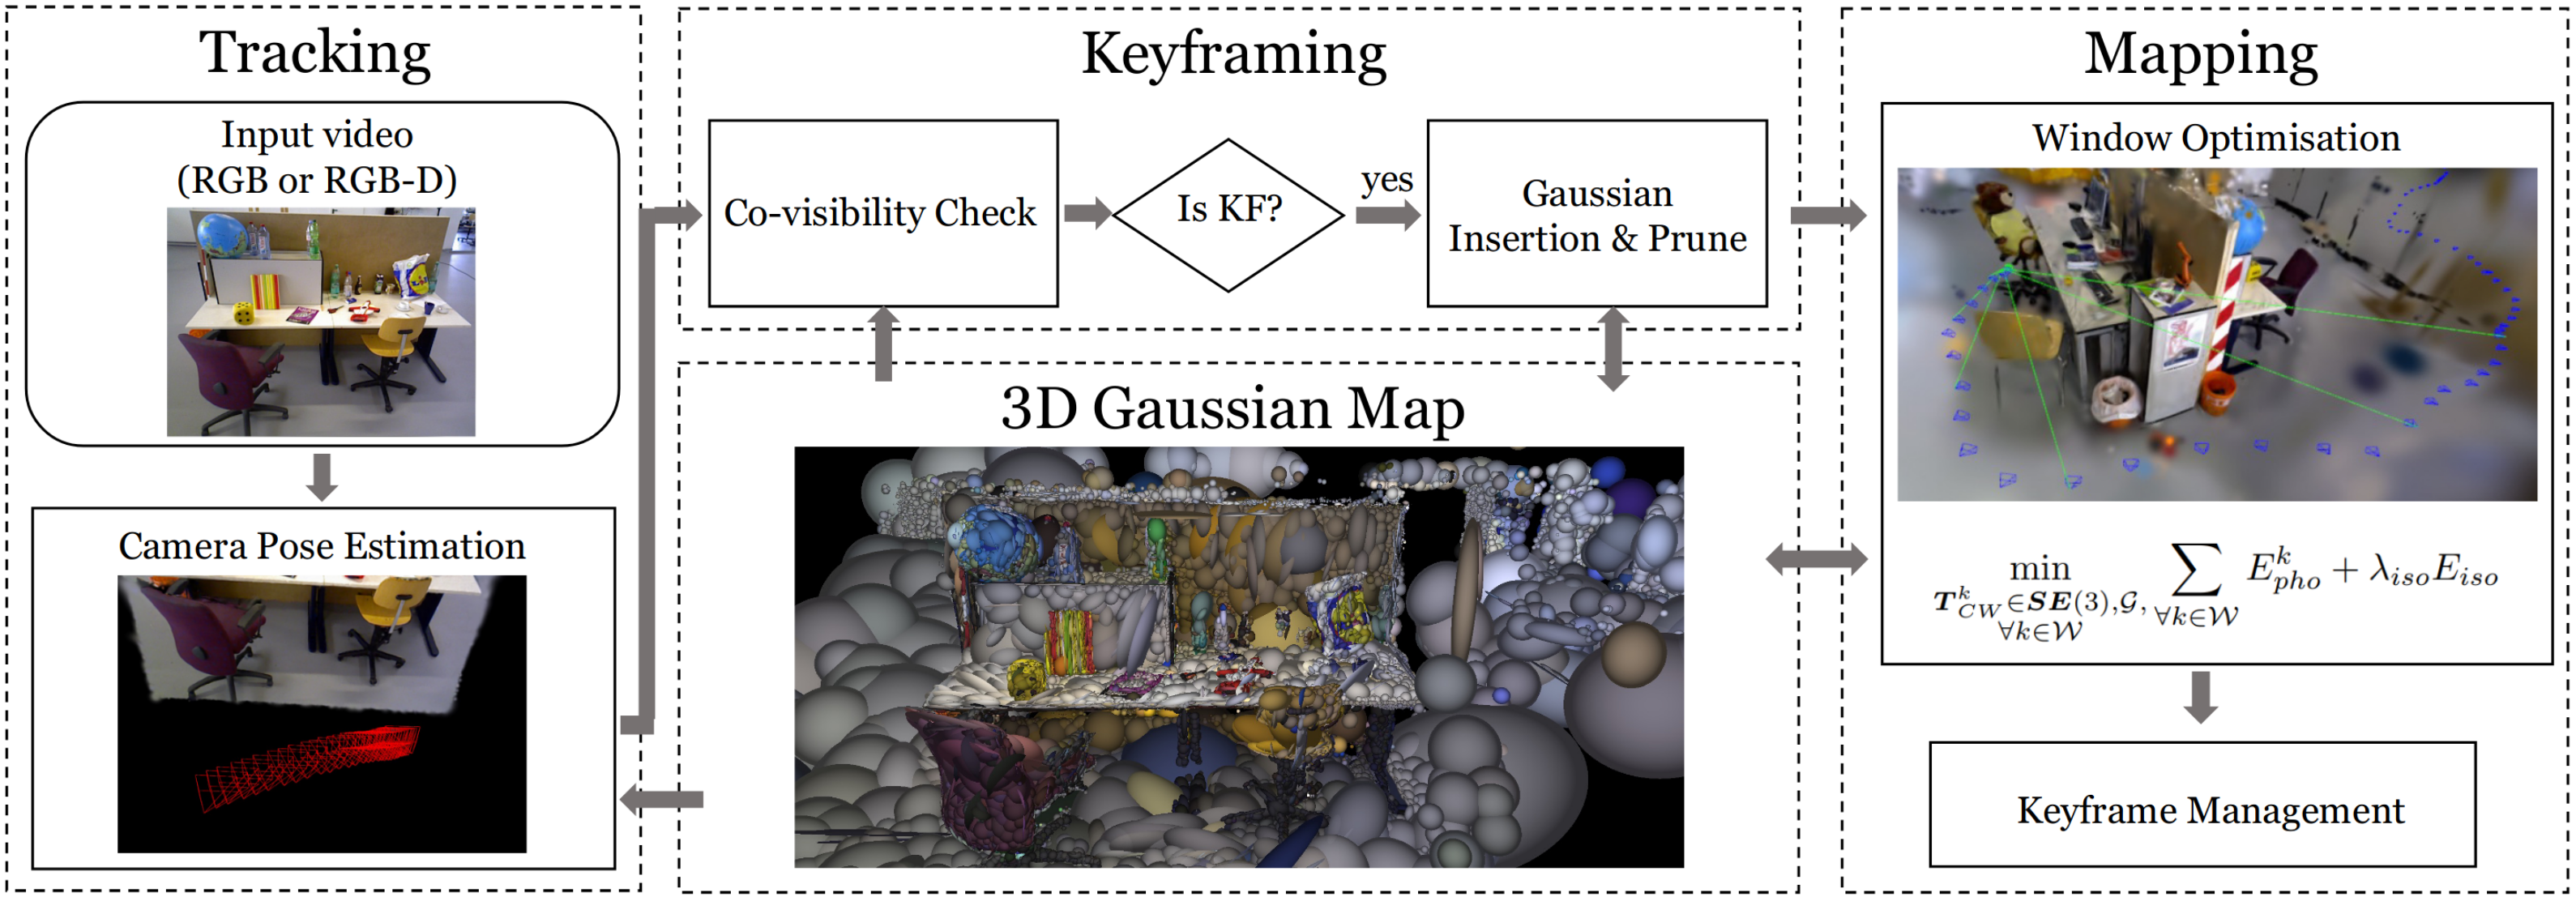
\includegraphics[width=\linewidth]{monogs/overview.png}
	\end{figure}
	\blfootnote{\href{http://arxiv.org/abs/2312.06741}{(CVPR Highlight, 2024) MonoGS: Gaussian Splatting SLAM}}
\end{Frame}

\tikzset{
	key/.style={
			draw=OrangeRed,
		},
	convention/.style={
			draw=Cerulean,
		},
	trick/.style={
			draw=ForestGreen,
		},
}
\begin{Frame}{Overview \romannum{2}}
	\centering
	\resizebox{0.85\textwidth}{!}{
		\begin{forest}
			for tree={my tree}
			[
			MonoGS
				[
					Visual Odometry,for children={visible on=<1->}
						[
							Tracking,for children={visible on=<2->}
								[
									``Inverse Rendering'',for children={visible on=<3->}
										[
											Analytical Jacobians Derivation,key
										]
										[
											Photometric RGB \& Depth Loss,convention
										]
										[
											Optimizable Exposure,trick
										]
										[
											Penalization on non-edge/low-opacity pixels,trick
										]
								]
						]
						[
							Mapping,for children={visible on=<2->}
								[
									Bundle Adjustment,for children={visible on=<3->}
										[
											Photometric RGB \& Depth Loss,convention
										]
										[
											Isotropic Regularization,key
										]
										[
											Random Recall,trick
										]
								]
						]
				]
				[
					Online Pipeline,for children={visible on=<1->}
						[
							Keyframe Management,for children={visible on=<2->}
								[
									Registration,for children={visible on=<3->}
										[
											Gaussian Covisibility,key
										]
										[
											Relative Translation,convention
										]
								]
								[
									Removal,for children={visible on=<3->}
										[
											Gaussian Overlap Coefficient,key
										]
								]
						]
						[
							Gaussian Management,for children={visible on=<2->}
								[
									Insertion,for children={visible on=<3->}
										[
											Keyframing,convention
										]
								]
								[
									Pruning,for children={visible on=<3->}
										[
											Gaussian Covisibility,key
										]
								]
						]
				]
			]
		\end{forest}
	}
	\resizebox{0.08\textwidth}{!}{
		\begin{tikzpicture}[visible on=<3->]
			\node [my node for tree, draw=ForestGreen] (trick node) {trick};
			\node [my node for tree, draw=OrangeRed, above of = trick node] {key method};
			\node [my node for tree, draw=Cerulean, below of = trick node] (convention) {convention};
		\end{tikzpicture}
	}
	\blfootnote{\href{http://arxiv.org/abs/2312.06741}{(CVPR Highlight, 2024) MonoGS: Gaussian Splatting SLAM}}
\end{Frame}

\begin{Frame}{Tracking: Overview}
	\begin{figure}[htbp]
		\centering
		\resizebox{0.7\textwidth}{!}{
			\begin{forest} for tree={my tree}
				[
				Tracking
				[
				``Inverse Rendering''
				[
				Analytical Jacobians Derivation,key
				]
				[
				Photometric RGB \& Depth Loss,convention
				]
				[
				Optimizable Exposure,trick
				]
				[
				Penalization on non-edge/low-opacity pixels,trick
				]
				]
				]
			\end{forest}
		}
	\end{figure}
	\vspace*{\fill}
	\par Track camera poses,
	\vspace*{1.5ex}
	\begin{itemize}[<+->]
		\setlength{\itemsep}{1.5ex}
		\item \textcolor{OrangeRed}{through the extended differentiable rendering pipeline},
		\item \textcolor{Cerulean}{by a direct optimization against fixed 3D Gaussians,}
		\item \textcolor{ForestGreen}{with some tricks to be more adaptive to brightness and more robust to noise.}
	\end{itemize}
	\blfootnote{
		\begin{tikzpicture}
			\node [inner sep=1pt, rounded corners=1.5, draw=ForestGreen] (trick node) {trick};
			\node [inner sep=1pt, rounded corners=1.5, draw=OrangeRed, left of = trick node] {key method};
			\node [inner sep=1pt, rounded corners=1.5, draw=Cerulean, right of = trick node] (convention) {convention};
		\end{tikzpicture}
	}
	\blfootnote{\href{http://arxiv.org/abs/2312.06741}{(CVPR Highlight, 2024) MonoGS: Gaussian Splatting SLAM}}
\end{Frame}

\begin{Frame}{Tracking: A Review of 3DGS}
	\vspace*{-5em}
	\par The projection from ``ellipsoids'' to ``ellipses'' in 3DGS,
	\begin{equation}
		\mathcal{N}\left(\mu_w, \Sigma_w\right) \overset{\pi}{\mapsto} \mathcal{N}\left(\mu_i, \Sigma_i\right),
	\end{equation}
	is achieved by,
	\begin{overprint}[\textheight]
		\begin{figure}[htbp]
			\centering
			\begin{minipage}[c]{0.35\linewidth}
				\resetcolorseries[4]{marknode-color-series}
				\resetcolorseries[4]{annotation-color-series}
				\begin{align}
					\alt<5->{\tikzmarknode{n3}{\colorbox{marknode-color-series!![3]}{\(\mu_{i}\)}}}{\mu_{i}}
					=
					\alt<4->{\tikzmarknode{n2}{\colorbox{marknode-color-series!![2]}{\(\pi\)}}}{\pi}
					\left(
					\alt<3->{\tikzmarknode{n1}{\colorbox{marknode-color-series!![1]}{\(\mathbf{T}_{cw}\)}}}{\mathbf{T}_{cw}}
					\cdot
					\alt<2->{\tikzmarknode{n0}{\colorbox{marknode-color-series!![0]}{\(\mu_{w}\)}}}{\mu_{w}}
					\right)
				\end{align}
				\begin{annotatedEquationEnv}
					\only<2->{\annotatedEquation{colorseries}{n0}{south}{0em}{-1em}{north west}{annotation-color-series}{\(\in \mathbb{P}^3\), 3D(world) mean}{east}}
					\only<3->{\annotatedEquation{colorseries}{n1}{south}{0em}{-3em}{north west}{annotation-color-series}{\(\in \mathrm{SE}(3)\), camera pose}{east}}
					\only<4->{\annotatedEquation{colorseries}{n2}{south}{0em}{-5em}{north west}{annotation-color-series}{projection}{east}}
					\only<5->{\annotatedEquation{colorseries}{n3}{south}{0}{-7em}{north west}{annotation-color-series}{\(\in \mathbb{P}^2\), 2D(image) mean}{east}}
				\end{annotatedEquationEnv}
			\end{minipage}
			\begin{minipage}[c]{0.60\linewidth}
				\resetcolorseries[4]{marknode-color-series}
				\resetcolorseries[4]{annotation-color-series}
				\begin{align}
					\alt<9->{\tikzmarknode{n3}{\colorbox{marknode-color-series!![3]}{\(\Sigma_{i}\)}}}{\Sigma_{i}}
					=
					\alt<8->{\tikzmarknode{n2}{\colorbox{marknode-color-series!![2]}{\(\mathbf{J}_{\pi}\)}}}{\mathbf{J}_{\pi}}
					\alt<7->{\tikzmarknode{n1}{\colorbox{marknode-color-series!![1]}{\(\mathbf{R}_{cw}\)}}}{\mathbf{R}_{cw}}
					\alt<6->{\tikzmarknode{n0}{\colorbox{marknode-color-series!![0]}{\(\Sigma_{w}\)}}}{\Sigma_{w}}  \mathbf{R}_{cw}^{\mathrm{T}} \mathbf{J}_{\pi}^{\mathrm{T}}
				\end{align}
				\begin{annotatedEquationEnv}
					\only<6->{\annotatedEquation{colorseries}{n0}{south}{0em}{-1em}{north west}{annotation-color-series}{\(\in \mathbb{R}^{3\times 3}\), 3D(world) covariance}{east}}
					\only<7->{\annotatedEquation{colorseries}{n1}{south}{0em}{-3em}{north west}{annotation-color-series}{\(\in \mathrm{SO(3)}\), rotation component of \(\mathbf{T}_{cw}\)}{east}}
					\only<8->{\annotatedEquation{colorseries}{n2}{south}{0em}{-5em}{north west}{annotation-color-series}{\(\in \mathbb{R}^{2\times 3}\), Jacobian of the linear approximation of \(\pi\)}{east}}
					\only<9->{\annotatedEquation{colorseries}{n3}{south}{0em}{-7em}{north west}{annotation-color-series}{\(\in \mathbb{R}^{2\times 2}\), 2D(image) covariance}{east}}
				\end{annotatedEquationEnv}
			\end{minipage}
		\end{figure}
	\end{overprint}
	\blfootnote{\href{http://arxiv.org/abs/2312.06741}{(CVPR Highlight, 2024) MonoGS: Gaussian Splatting SLAM}}
\end{Frame}

\begin{Frame}{Tracking: Derivation of Jacobians \romannum{1}}
	\par The chain rule,
	\begin{alignat}{1}
		\frac{\partial \mu_i}{\partial \mathbf{T}_{cw}}    & = \frac{\partial \mu_i}{\partial \mu_c} \frac{\partial \mu_c}{\partial \mathbf{T}_{cw}}                                                                                                                                                                               \\
		\frac{\partial \Sigma_i}{\partial \mathbf{T}_{cw}} & = \frac{\partial \Sigma_i}{\partial \mathbf{J}_{\pi}} \frac{\partial \mathbf{J}_{\pi}}{\partial \mu_c} \frac{\partial \mu_c}{\partial \mathbf{T}_{cw}} + \frac{\partial \Sigma_i}{\partial \mathbf{R}_{cw}} \frac{\partial \mathbf{R}_{cw}}{\partial \mathbf{T}_{cw}}
	\end{alignat}
	\pause
	\par The Lie Algebra,
	\begin{alignat}{1}
		\frac{\partial \mu_c}{\partial \mathbf{T}_{cw}}           & = \begin{bmatrix}
			                                                              \mathbf{I} & -\mu_{c}^{\times}
		                                                              \end{bmatrix}               \\
		\frac{\partial \mathbf{R}_{cw}}{\partial \mathbf{T}_{cw}} & = \begin{bmatrix}
			                                                              \mathbf{0} & - \mathbf{R}_{cw}^{\times}(:,1) \\
			                                                              \mathbf{0} & - \mathbf{R}_{cw}^{\times}(:,2) \\
			                                                              \mathbf{0} & - \mathbf{R}_{cw}^{\times}(:,3) \\
		                                                              \end{bmatrix}
	\end{alignat}
	\blfootnote{\href{http://arxiv.org/abs/2312.06741}{(CVPR Highlight, 2024) MonoGS: Gaussian Splatting SLAM}}
\end{Frame}

\begin{Frame}{Online Pipeline: Overview}
	\begin{figure}[htbp]
		\centering
		\resizebox{0.8\textwidth}{!}{
			\begin{forest}
				for tree={my tree}
				[
				Online Pipeline
					[
						Keyframe Management
							[
								Registration
									[
										Gaussian Covisibility,key
									]
									[
										Relative Translation,convention
									]
							]
							[
								Removal
									[
										Gaussian Overlap Coefficient,key
									]
							]
					]
					[
						Gaussian Management
							[
								Insertion
									[
										Keyframing,convention
									]
							]
							[
								Pruning
									[
										Gaussian Covisibility,key
									]
							]
					]
				]
			\end{forest}
		}
	\end{figure}
	\par \alert<+|handout:0>{Keyframe Management}:
	\vspace*{1.5ex}
	\begin{itemize}[<+->]
		\setlength{\itemsep}{1.5ex}
		\item \alert<.|handout:0>{Classic} strategies, e.g. covisibility \& overlap, from DSO~\autocite{engel2016dso}.
		\item \alert<.|handout:0>{Off-the-shelf} occlusion-aware Gaussian visibility is leveraged to construct metrics.
	\end{itemize}
	\blfootnote{
		\begin{tikzpicture}
			\node [inner sep=1pt, rounded corners=1.5, draw=ForestGreen] (trick node) {trick};
			\node [inner sep=1pt, rounded corners=1.5, draw=OrangeRed, left of = trick node] {key method};
			\node [inner sep=1pt, rounded corners=1.5, draw=Cerulean, right of = trick node] (convention) {convention};
		\end{tikzpicture}
	}
	\blfootnote{\href{http://arxiv.org/abs/1607.02565}{(arXiv, 2016) DSO: Direct Sparse Odometry}}
	\blfootnote{\href{http://arxiv.org/abs/2312.06741}{(CVPR Highlight, 2024) MonoGS: Gaussian Splatting SLAM}}
\end{Frame}

\begin{Frame}{Online Pipeline: Overview}
	\begin{figure}[htbp]
		\centering
		\resizebox{0.8\textwidth}{!}{
			\begin{forest}
				for tree={my tree}
				[
				Online Pipeline
					[
						Keyframe Management
							[
								Registration
									[
										Gaussian Covisibility,key
									]
									[
										Relative Translation,convention
									]
							]
							[
								Removal
									[
										Gaussian Overlap Coefficient,key
									]
							]
					]
					[
						Gaussian Management
							[
								Insertion
									[
										Keyframing,convention
									]
							]
							[
								Pruning
									[
										Gaussian Covisibility,key
									]
							]
					]
				]
			\end{forest}
		}
	\end{figure}
	\par \alert<+|handout:0>{Gaussian Management:}
	\vspace*{1.5ex}
	\begin{itemize}[<+->]
		\setlength{\itemsep}{1.5ex}
		\item \alert<.>{Insertion:} triggered by \alert<.>{keyframing}, followed by \alert<.>{Gaussian initialization}.
		\item \alert<.>{Pruning:} to remove unstable/incorrect Gaussians by covisibility in a monocular setting.
	\end{itemize}
	\blfootnote{
		\begin{tikzpicture}
			\node [inner sep=1pt, rounded corners=1.5, draw=ForestGreen] (trick node) {trick};
			\node [inner sep=1pt, rounded corners=1.5, draw=OrangeRed, left of = trick node] {key method};
			\node [inner sep=1pt, rounded corners=1.5, draw=Cerulean, right of = trick node] (convention) {convention};
		\end{tikzpicture}
	}
	\blfootnote{\href{http://arxiv.org/abs/1607.02565}{(arXiv, 2016) DSO: Direct Sparse Odometry}}
	\blfootnote{\href{http://arxiv.org/abs/2312.06741}{(CVPR Highlight, 2024) MonoGS: Gaussian Splatting SLAM}}
\end{Frame}

\begin{Frame}{Keyframe Management: Prerequistes}
	\begin{enumerate}
		\setlength{\itemsep}{3ex}
		\item<+-> \alert<.>{What} is keyframing or keyframe management?
			\vspace*{1.5ex}
			\begin{itemize}
				\setlength{\itemsep}{1.5ex}
				\item<+-> A strategy of \alert<.>{selecting} and \alert<.>{utilizing} a \alert<.>{crucial subset} of frames.
			\end{itemize}
		\item<+-> \alert<.>{Why} do we need keyframing?
			\vspace*{1.5ex}
			\begin{itemize}
				\setlength{\itemsep}{1.5ex}
				\item<+-> \alert<.>{Infeasible} to optimize jointly on all frames online.
					\vspace*{1.5ex}
					\visible<+->{\par (a \alert<.>{trade-off} between efficiency and accuracy/robustness/...)}
			\end{itemize}
		\item<+-> \alert<.>{How} should we select keyframes?
			\vspace*{1.5ex}
			\begin{itemize}
				\setlength{\itemsep}{1.5ex}
				\item<+-> \alert<.>{non-redundant} and observing the \alert<.>{same area}.
				\item<+-> spanning a \alert<.>{wide baseline} for better multi-view constraints.
			\end{itemize}
	\end{enumerate}
	\blfootnote{\href{http://arxiv.org/abs/2312.06741}{(CVPR Highlight, 2024) MonoGS: Gaussian Splatting SLAM}}
\end{Frame}

\begin{Frame}{Keyframe Management: Registration}
	\blfootnote{\href{http://arxiv.org/abs/2312.06741}{(CVPR Highlight, 2024) MonoGS: Gaussian Splatting SLAM}}
	\begin{overprint}[\textheight]
		\par If \alert<+>{any} of the following conditions \alert<.>{is true}...
		\vspace*{\fill}
		\resetcolorseries[6]{marknode-color-series}
		\resetcolorseries[6]{annotation-color-series}
		\begin{block}<+->{\alert<.|handout:0>{Small Gaussian Covisibility}\hfill Condition \romannum{1}, Keyframe Registration}
			Gaussian covisibility between the current frame and the previous keyframe drops below a threshold.
			\begin{figure}[htbp]
				\centering
				\begin{onlyenv}<.>
					\vspace*{-2em}
					\begin{equation*}
						\frac{\vert\operatorname{v}\left(\mathcal{G}, \mathcal{F}_{i}\right) \cap \tikzmarknode{n0}{\colorbox{marknode-color-series!![0]}{\(\operatorname{v}\left(\mathcal{G}, \mathcal{F}_{j}\right)\)}} \vert}{\vert\operatorname{v}\left(\mathcal{G}, \tikzmarknode{n1}{\colorbox{marknode-color-series!![1]}{\(\mathcal{F}_{i}\)}}\right) \cup \operatorname{v}\left(\mathcal{G}, \tikzmarknode{n2}{\colorbox{marknode-color-series!![2]}{\(\mathcal{F}_{j}\)}}\right) \vert} < \tau_1
					\end{equation*}
					\begin{annotatedEquationEnv}
						\annotatedEquation{colorseries}{n0}{north}{0em}{1em}{south west}{annotation-color-series}{\(\subset \mathcal{G}\), \textbf{visible} Gaussians from frame \(j\)}{east}
						\annotatedEquation{colorseries}{n1}{south}{0em}{-0.5em}{north east}{annotation-color-series}{the previous keyframe}{west}
						\annotatedEquation{colorseries}{n2}{south}{0em}{-0.5em}{north west}{annotation-color-series}{the current frame}{east}
					\end{annotatedEquationEnv}
				\end{onlyenv}
				\begin{onlyenv}<+-|handout:0>
					\vspace*{-2em}
					\begin{equation}
						\frac{\vert\operatorname{v}\left(\mathcal{G}, \mathcal{F}_{i}\right) \cap \operatorname{v}\left(\mathcal{G}, \mathcal{F}_{j}\right) \vert}{\vert\operatorname{v}\left(\mathcal{G}, \mathcal{F}_{i}\right) \cup \operatorname{v}\left(\mathcal{G}, \mathcal{F}_{j}\right) \vert} < \tau_1
					\end{equation}
					\vspace*{-2em}
				\end{onlyenv}
			\end{figure}
		\end{block}
		\vspace*{\fill}
		\begin{block}<.->{\alert<.|handout:0>{Large Relative Translation}\hfill Condition \romannum{2}, Keyframe Registration}
			Translation from the previous keyframe w.r.t. to the median depth reaches a threshold.
			\begin{figure}[htbp]
				\centering
				\vspace*{-2em}
				\begin{onlyenv}<.>
					\begin{equation*}
						\frac{\Vert \mathbf{t}_{\mathcal{F}_i \mathcal{F}_j} \Vert_2}{\bar{D}_{\mathcal{F}_i \mathcal{F}_j}} > \tau_2, \quad \bar{D}_{\mathcal{F}_i \mathcal{F}_j} = \frac{1}{2 \tikzmarknode{n4}{\colorbox{marknode-color-series!![4]}{\(H\)}} \tikzmarknode{n5}{\colorbox{marknode-color-series!![5]}{\(W\)}}} \sum^{\{\mathcal{F}_i,\mathcal{F}_j\}} \sum_{h=0}^{H} \sum_{w=0}^{W} \tikzmarknode{n3}{\colorbox{marknode-color-series!![3]}{\(d(h,w)\)}}
					\end{equation*}
					\begin{annotatedEquationEnv}
						\annotatedEquation{colorseries}{n3}{south}{0}{-0.5em}{north west}{annotation-color-series}{depth of pixel \((h,w)\)}{east}
						\annotatedEquation{colorseries}{n4}{south}{0}{-0.5em}{north east}{annotation-color-series}{image height}{west}
						\annotatedEquation{colorseries}{n5}{south}{0}{-0.5em}{north west}{annotation-color-series}{image width}{east}
					\end{annotatedEquationEnv}
				\end{onlyenv}
				\begin{onlyenv}<+-|handout:0>
					\begin{equation}
						\frac{\Vert \mathbf{t}_{\mathcal{F}_i \mathcal{F}_j} \Vert_2}{\bar{D}_{\mathcal{F}_i \mathcal{F}_j}} > \tau_2, \quad \bar{D}_{\mathcal{F}_i \mathcal{F}_j} = \frac{1}{2 H W} \sum^{\{\mathcal{F}_i,\mathcal{F}_j\}} \sum_{h=0}^{H} \sum_{w=0}^{W} d(h,w)
					\end{equation}
					\vspace*{-2em}
				\end{onlyenv}
			\end{figure}
		\end{block}
	\end{overprint}
\end{Frame}

\begin{Frame}{Keyframe Management: Removal}
	\blfootnote{\href{http://arxiv.org/abs/2312.06741}{(CVPR Highlight, 2024) MonoGS: Gaussian Splatting SLAM}}
	\begin{overprint}[\textheight]
		\par If \alert<+>{any} of the following conditions \alert<.>{is true}...
		\vspace*{\fill}
		\begin{block}{\alert<.|handout:0>{Beyond Window Capacity}\hfill Condition \romannum{1}, Keyframe Removal}<+->
			Remove the earliest keyframe out of the sliding window if the capacity is exceeded.
			\begin{equation}
				\vert \mathcal{W} \vert < \tau_3
			\end{equation}
		\end{block}
		\vspace*{\fill}
		\begin{block}{\alert<.|handout:0>{Low Gaussian Overlap Coefficient}\hfill Condition \romannum{2}, Keyframe Removal}<+->
			Remove the previous keyframe if the ``Gaussian overlap coefficient'' between the previous frame and the new keyframe drops below a threshold.
			\begin{equation}
				\frac{\vert \operatorname{v}\left(\mathcal{G}, \mathcal{F}_{i}\right) \cap \operatorname{v}\left(\mathcal{G}, \mathcal{F}_{j}\right) \vert}{\min \left(\vert\operatorname{v}\left(\mathcal{G}, \mathcal{F}_{i}\right) \vert, \vert\operatorname{v}\left(\mathcal{G}, \mathcal{F}_{j}\right) \vert\right)} < \tau_4
			\end{equation}
		\end{block}
	\end{overprint}
\end{Frame}

\begin{Frame}{Gaussian Management: Insertion}
	\begin{itemize}
		\setlength{\itemsep}{1.5ex}
		\item<+-> \alert<.>{Why} do we need ``Gaussian insertion''?
			\vspace*{1.5ex}
			\begin{itemize}
				\setlength{\itemsep}{1.5ex}
				\item<+-> \alert<.>{SLAM} is for robotic exploration.
			\end{itemize}
	\end{itemize}
	\vspace*{\fill}
	\begin{itemize}
		\setlength{\itemsep}{1.5ex}
		\item<+-> \alert<.>{When} do we need ``Gaussian insertion''?
	\end{itemize}
	\begin{block}{\alert<.|handout:0>{Keyframing}\hfill Condition \romannum{1}, Gaussian Insertion}<+->
		\par Insertion is triggered for every new keyframe.
	\end{block}
	\blfootnote{\href{http://arxiv.org/abs/2312.06741}{(CVPR Highlight, 2024) MonoGS: Gaussian Splatting SLAM}}
\end{Frame}

\begin{Frame}{Gaussian Management: Initialization}
	\begin{itemize}
		\setlength{\itemsep}{1.5ex}
		\item<+-> \alert<.>{How} do we insert Gaussians?
			\vspace*{1.5ex}
			\begin{itemize}
				\setlength{\itemsep}{1.5ex}
				\item<+-> Gaussian insertion is Gaussian \alert<.>{initialization}.
			\end{itemize}
	\end{itemize}
	\vspace*{\fill}
	\begin{block}{\alert<.|handout:0>{If Depth Available}\hfill Gaussian Initialization}<+->
		Back-project in a per-pixel, per-Gaussian approach.
	\end{block}
	\vspace*{\fill}
	\begin{block}{\alert<.|handout:0>{If Depth Unavailable}\hfill Gaussian Initialization}<+->
		Leverage the rendered depth map.
		\vspace*{1.5ex}
		\begin{itemize}[<+->]
			\setlength{\itemsep}{1.5ex}
			\item \alert<.|handout:0>{for pixels with depth:} use the rendered depth and assign a ``low'' covariance.
			\item \alert<.|handout:0>{for pixels w/o depth:} use the median of rendered depth and assign a ``high'' covariance.
		\end{itemize}
	\end{block}
	\blfootnote{
		In practice, ``low'': \(\sf 0.2 \sigma \); ``high'': \(0.5 \sigma\), where \(\sigma\) is the standard deviation of the rendered depth map.
	}
	\blfootnote{\href{http://arxiv.org/abs/2312.06741}{(CVPR Highlight, 2024) MonoGS: Gaussian Splatting SLAM}}
\end{Frame}

\begin{Frame}{Gaussian Management: Pruning}
	\begin{itemize}
		\setlength{\itemsep}{1.5ex}
		\item<+-> \alert<.>{Why} do we need ``Gaussian Pruning'' \textbf{if depth unavailable}?
			\vspace*{1.5ex}
			\begin{itemize}
				\setlength{\itemsep}{1.5ex}
				\item<+-> Too many \alert<.>{incorrect/unstable} newly inserted Gaussians.
			\end{itemize}
	\end{itemize}
	\vspace*{\fill}
	\begin{block}{\alert<.|handout:0>{Low Gaussian Opacity} \hfill Condition \romannum{1}, Gaussian Pruning}<+->
		The Gaussians with a ``low'' opacity are pruned.
	\end{block}
	\vspace*{\fill}
	\begin{block}{\alert<.|handout:0>{Low Gaussian Covisibility} \hfill Condition \romannum{2}, Gaussian Pruning}<+->
		For ``just'' inserted Gaussians but unobserved by ``some other'' keyframes, are pruned out.
	\end{block}
	\blfootnote{If no pruning, although the majority of incorrect Gaussians vanish quickly in following optimization, there are some survivals.}
	\blfootnote{In practice, the opacity threshold is \(\sf 0.7\).}
	\blfootnote{In practice, the pruned Gaussians are inserted in the last 3 keyframes and unobserved by any other 3 keyframes in the sliding window.}
	\blfootnote{\href{http://arxiv.org/abs/2312.06741}{(CVPR Highlight, 2024) MonoGS: Gaussian Splatting SLAM}}
\end{Frame}

\begin{Frame}{Mapping: Overview}
	\begin{center}
		\resizebox{!}{0.25\textheight}{
			\begin{forest}
				for tree={my tree}
				[
				Mapping
					[
						Bundle Adjustment
							[
								Photometric RGB \& Depth Loss,convention
							]
							[
								Isotropic Regularization,key
							]
							[
								Random Recall,trick
							]
					]
				]
			\end{forest}
		}
	\end{center}
	\pause
	\vspace*{\fill}
	\begin{itemize}
		\setlength{\itemsep}{1.5ex}
		\item<+-> \alert<.>{Why} do we need mapping in \textbf{3DGS} SLAM?
			\vspace*{1.5ex}
			\begin{itemize}
				\setlength{\itemsep}{1.5ex}
				\item<+-> \alert<.|handout:0>{Local Mapping}: Optimize newly inserted 3D Gaussians.
				\item<+-> \alert<.|handout:0>{Global Mapping}: Reconstruct a 3D-coherent structure.
			\end{itemize}
	\end{itemize}
	\blfootnote{
		\begin{tikzpicture}
			\node [inner sep=1pt, rounded corners=1.5, draw=ForestGreen] (trick node) {trick};
			\node [inner sep=1pt, rounded corners=1.5, draw=OrangeRed, left of = trick node] {key method};
			\node [inner sep=1pt, rounded corners=1.5, draw=Cerulean, right of = trick node] (convention) {convention};
		\end{tikzpicture}
	}
	\blfootnote{\href{http://arxiv.org/abs/2312.06741}{(CVPR Highlight, 2024) MonoGS: Gaussian Splatting SLAM}}
\end{Frame}

\begin{Frame}{Mapping: Bundle Adjustment \& Random Recall}
	\begin{block}<+->{\alert<.|handout:0>{Bundle Adjustment}}
		\begin{figure}[htbp]
			\centering
			\resetcolorseries[1]{marknode-color-series}
			\resetcolorseries[1]{annotation-color-series}
			\begin{equation}
				\underset{\mathcal{G}, \{\mathbf{T}_{cw}({\mathcal{F}_k})\vert \mathcal{F}_k\in \mathcal{W}\}}{\operatorname{argmin}} \sum_{\mathcal{F}_k}^{\tikzmarknode{n0}{\colorbox{marknode-color-series!![0]}{\scriptsize\(\mathcal{W}\)}}} \mathcal{L}_{pho}\left({\mathcal{F}_k}\right)
			\end{equation}
			\begin{annotatedEquationEnv}
				\annotatedEquation{colorseries}{n0}{north}{0em}{+0.5em}{south west}{annotation-color-series}{keyframes in the sliding window}{east}
			\end{annotatedEquationEnv}
		\end{figure}
		\vspace*{-1.5ex}
	\end{block}
	\vspace*{\fill}
	\begin{block}<+->{\alert<.|handout:0>{Random Recall} \hfill A trick for global mapping}
		\vspace*{0.5ex}
		\par Besides \(\mathcal{W}\), ``some'' randomly selected past keyframes are also leveraged in BA to avoid forgetting the global map.
	\end{block}
	\blfootnote{\href{http://arxiv.org/abs/2312.06741}{(CVPR Highlight, 2024) MonoGS: Gaussian Splatting SLAM}}
\end{Frame}

\begin{Frame}{Mapping: Isotropic Regularization}
	\begin{itemize}
		\setlength{\itemsep}{1.5ex}
		\item<+-> \alert<.>{Why} do we need ``isotropic regularization''?
			\vspace*{1.5ex}
			\begin{itemize}
				\setlength{\itemsep}{1.5ex}
				\item<+-> \alert<.|handout:0>{Observation:} isotropic Gaussians behave better than anisotrophic.
				\item<+-> \alert<.|handout:0>{Analysis:} no constraints on the elongation along the viewing ray direction, \textbf{even with depth}.
			\end{itemize}
	\end{itemize}
	\vspace*{\fill}
	\begin{block}<+->{\alert<.|handout:0>{Isotropic Regularization}}
		\vspace*{0.5ex}
		\begin{equation}
			\mathcal{L}_{iso} = \sum_{i=1}^{\vert \mathcal{G} \vert} \Vert \mathbf{s}_i - \bar{\mathbf{s}}_i \Vert_1, \quad\text{where } \bar{\mathbf{s}}_i = \frac{1}{3} \left( s_i^{x} + s_i^{y} + s_i^{z} \right).
		\end{equation}
	\end{block}
	\blfootnote{\href{http://arxiv.org/abs/2312.06741}{(CVPR Highlight, 2024) MonoGS: Gaussian Splatting SLAM}}
\end{Frame}

\begin{Frame}{Mapping: Conclusion}
	\begin{block}{The Overall Optimization for Mapping}
		\begin{equation}
			\underset{\mathcal{G}, \{\mathbf{T}_{cw}({\mathcal{F}_k})\vert \mathcal{F}_k\in \mathcal{W}^{+}\}}{\operatorname{argmin}} \sum_{\mathcal{F}_k}^{\mathcal{W}^{+}} \mathcal{L}_{pho}\left({\mathcal{F}_k}\right) + \lambda_{iso} \mathcal{L}_{iso}
		\end{equation}
	\end{block}
	\blfootnote{\href{http://arxiv.org/abs/2312.06741}{(CVPR Highlight, 2024) MonoGS: Gaussian Splatting SLAM}}
\end{Frame}


\appendix

\section{\appendixname}

\subsection{References}

\begin{frame}[allowframebreaks]
	\frametitle{References}
	% \nocite{*}
	\printbibliography[heading=none]
\end{frame}

\end{document}

